\documentclass[tikz,border=15pt]{standalone}
\usepackage{tikz}
\usepackage{xcolor}
\usetikzlibrary{arrows.meta,calc}

\definecolor{bgcolor}{RGB}{11,17,32}
\definecolor{cardbg}{RGB}{30,41,59}
\definecolor{cardborder}{RGB}{51,65,85}
\definecolor{clientborder}{RGB}{56,189,248}
\definecolor{clientbg}{RGB}{23,37,84}
\definecolor{pepborder}{RGB}{14,165,233}
\definecolor{pepbg}{RGB}{7,89,133}
\definecolor{stsborder}{RGB}{192,132,252}
\definecolor{stsbg}{RGB}{76,29,149}
\definecolor{pdpborder}{RGB}{251,191,36}
\definecolor{pdpbg}{RGB}{120,53,15}
\definecolor{resborder}{RGB}{52,211,153}
\definecolor{resbg}{RGB}{6,78,59}
\definecolor{slategray}{RGB}{148,163,184}

\begin{document}
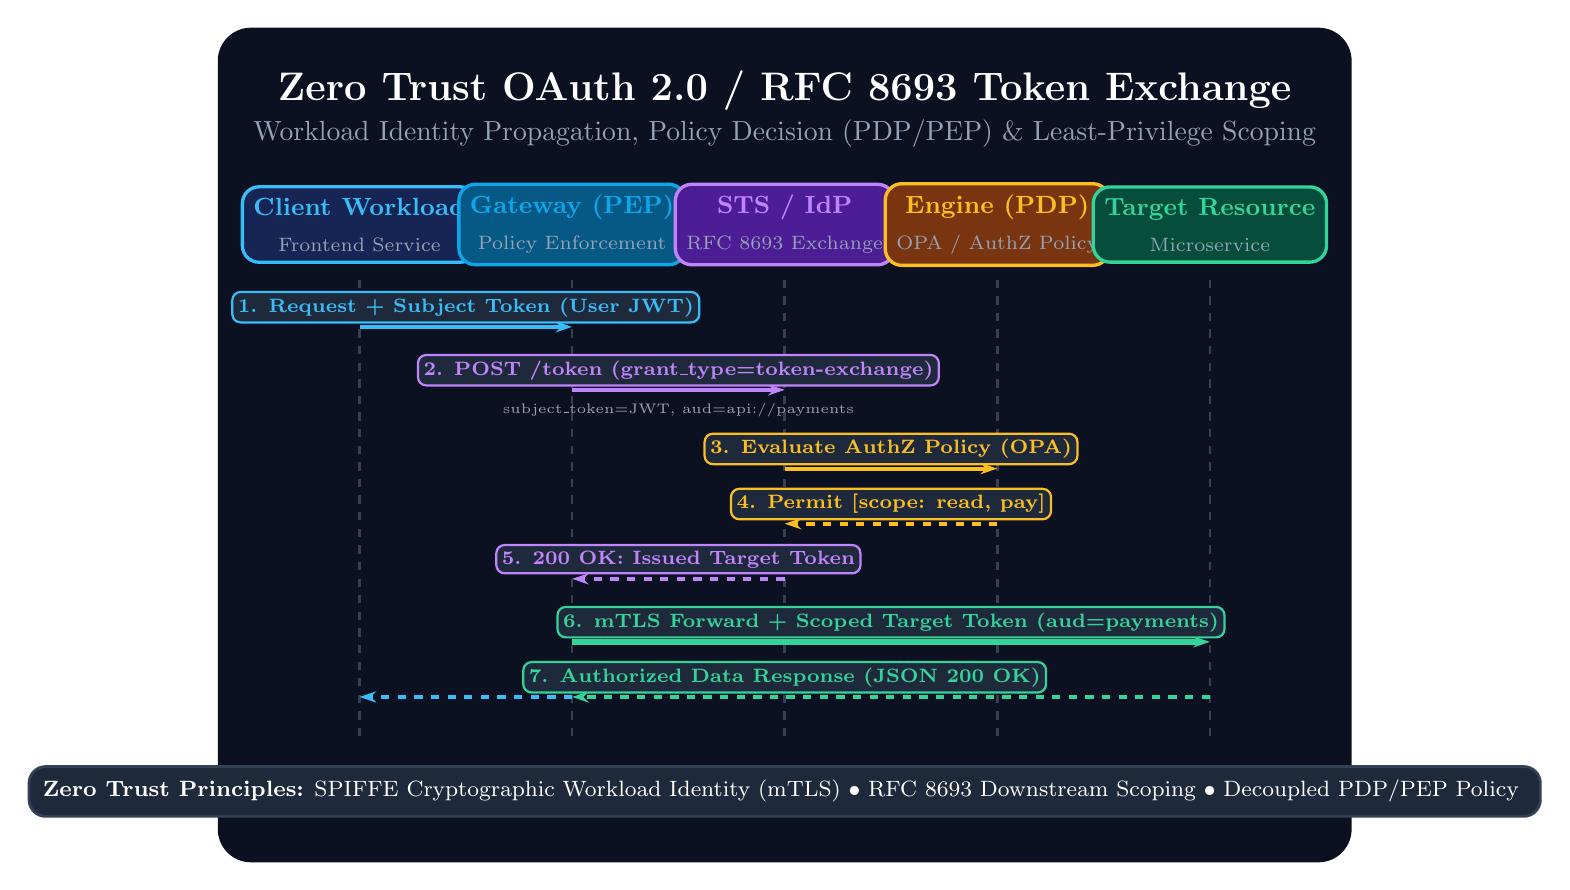
\begin{tikzpicture}[
    >={Stealth[length=6pt, width=4pt]}
]

% Background Card
\fill[rounded corners=12pt, fill=bgcolor] (-7.2,-5.4) rectangle (7.2,5.2);

% Title & Header
\node[text=white, font=\Large\bfseries] at (0, 4.4) {Zero Trust OAuth 2.0 / RFC 8693 Token Exchange};
\node[text=slategray, font=\normalsize] at (0, 3.85) {Workload Identity Propagation, Policy Decision (PDP/PEP) \& Least-Privilege Scoping};

% ACTOR COLUMNS
% 1: Client at x = -5.4
% 2: PEP Gateway at x = -2.7
% 3: STS at x = 0.0
% 4: PDP at x = 2.7
% 5: Target Resource at x = 5.4

\def\cOne{-5.4}
\def\cTwo{-2.7}
\def\cThree{0.0}
\def\cFour{2.7}
\def\cFive{5.4}

% Actor Headers
\node[fill=clientbg, draw=clientborder, line width=1.2pt, rounded corners=6pt, text=white, font=\small, align=center, inner sep=4pt] (H1) at (\cOne, 2.7) {
    \textbf{\textcolor{clientborder}{Client Workload}}\\[2pt]
    \textcolor{slategray}{\scriptsize Frontend Service}
};

\node[fill=pepbg, draw=pepborder, line width=1.2pt, rounded corners=6pt, text=white, font=\small, align=center, inner sep=4pt] (H2) at (\cTwo, 2.7) {
    \textbf{\textcolor{pepborder}{Gateway (PEP)}}\\[2pt]
    \textcolor{slategray}{\scriptsize Policy Enforcement}
};

\node[fill=stsbg, draw=stsborder, line width=1.2pt, rounded corners=6pt, text=white, font=\small, align=center, inner sep=4pt] (H3) at (\cThree, 2.7) {
    \textbf{\textcolor{stsborder}{STS / IdP}}\\[2pt]
    \textcolor{slategray}{\scriptsize RFC 8693 Exchange}
};

\node[fill=pdpbg, draw=pdpborder, line width=1.2pt, rounded corners=6pt, text=white, font=\small, align=center, inner sep=4pt] (H4) at (\cFour, 2.7) {
    \textbf{\textcolor{pdpborder}{Engine (PDP)}}\\[2pt]
    \textcolor{slategray}{\scriptsize OPA / AuthZ Policy}
};

\node[fill=resbg, draw=resborder, line width=1.2pt, rounded corners=6pt, text=white, font=\small, align=center, inner sep=4pt] (H5) at (\cFive, 2.7) {
    \textbf{\textcolor{resborder}{Target Resource}}\\[2pt]
    \textcolor{slategray}{\scriptsize Microservice}
};

% Vertical Lifelines
\draw[cardborder, dashed, line width=1pt] (\cOne, 2.0) -- (\cOne, -3.8);
\draw[cardborder, dashed, line width=1pt] (\cTwo, 2.0) -- (\cTwo, -3.8);
\draw[cardborder, dashed, line width=1pt] (\cThree, 2.0) -- (\cThree, -3.8);
\draw[cardborder, dashed, line width=1pt] (\cFour, 2.0) -- (\cFour, -3.8);
\draw[cardborder, dashed, line width=1pt] (\cFive, 2.0) -- (\cFive, -3.8);

% SEQUENCE FLOW STEPS
% Step 1: Client -> PEP
\draw[clientborder, line width=1.5pt, ->] (\cOne, 1.4) -- (\cTwo, 1.4);
\node[fill=cardbg, draw=clientborder, line width=0.8pt, rounded corners=3pt, text=clientborder, font=\scriptsize\bfseries, inner sep=2pt] at (-4.05, 1.65) {1. Request + Subject Token (User JWT)};

% Step 2: PEP -> STS
\draw[stsborder, line width=1.5pt, ->] (\cTwo, 0.6) -- (\cThree, 0.6);
\node[fill=cardbg, draw=stsborder, line width=0.8pt, rounded corners=3pt, text=stsborder, font=\scriptsize\bfseries, inner sep=2pt] at (-1.35, 0.85) {2. POST /token (grant\_type=token-exchange)};
\node[text=slategray, font=\tiny] at (-1.35, 0.35) {subject\_token=JWT, aud=api://payments};

% Step 3: STS -> PDP
\draw[pdpborder, line width=1.5pt, ->] (\cThree, -0.4) -- (\cFour, -0.4);
\node[fill=cardbg, draw=pdpborder, line width=0.8pt, rounded corners=3pt, text=pdpborder, font=\scriptsize\bfseries, inner sep=2pt] at (1.35, -0.15) {3. Evaluate AuthZ Policy (OPA)};

% Step 4: PDP -> STS
\draw[pdpborder, dashed, line width=1.5pt, ->] (\cFour, -1.1) -- (\cThree, -1.1);
\node[fill=cardbg, draw=pdpborder, line width=0.8pt, rounded corners=3pt, text=pdpborder, font=\scriptsize\bfseries, inner sep=2pt] at (1.35, -0.85) {4. Permit [scope: read, pay]};

% Step 5: STS -> PEP
\draw[stsborder, dashed, line width=1.5pt, ->] (\cThree, -1.8) -- (\cTwo, -1.8);
\node[fill=cardbg, draw=stsborder, line width=0.8pt, rounded corners=3pt, text=stsborder, font=\scriptsize\bfseries, inner sep=2pt] at (-1.35, -1.55) {5. 200 OK: Issued Target Token};

% Step 6: PEP -> Target Resource
\draw[resborder, line width=2pt, ->] (\cTwo, -2.6) -- (\cFive, -2.6);
\node[fill=cardbg, draw=resborder, line width=0.8pt, rounded corners=3pt, text=resborder, font=\scriptsize\bfseries, inner sep=2pt] at (1.35, -2.35) {6. mTLS Forward + Scoped Target Token (aud=payments)};

% Step 7: Target -> PEP -> Client
\draw[resborder, dashed, line width=1.5pt, ->] (\cFive, -3.3) -- (\cTwo, -3.3);
\draw[clientborder, dashed, line width=1.5pt, ->] (\cTwo, -3.3) -- (\cOne, -3.3);
\node[fill=cardbg, draw=resborder, line width=0.8pt, rounded corners=3pt, text=resborder, font=\scriptsize\bfseries, inner sep=2pt] at (0.0, -3.05) {7. Authorized Data Response (JSON 200 OK)};

% Summary Bottom Box
\node[fill=cardbg, draw=cardborder, line width=1pt, rounded corners=6pt, text=white, font=\footnotesize, align=center, inner sep=5pt] at (0, -4.5) {
    \textbf{Zero Trust Principles:} SPIFFE Cryptographic Workload Identity (mTLS) $\bullet$ RFC 8693 Downstream Scoping $\bullet$ Decoupled PDP/PEP Policy
};

\end{tikzpicture}
\end{document}
